\chapter{Technology Review}
\section{Game engines}
In this chapter, I will be delving into the advantages and disadvantages of the technology I picked relative to the alternatives and ultimately the reasons why I picked Unity as my game development engine. The two game engines that I looked at were the Unity game engine and the Unreal game engine.
\subsection{Overview of Unity}
The Unity game engine is a game development engine created by Unity Technologies. It supports the creation of both 2-dimensional and 3-dimensional applications for over 20 different \cite{UnitySupportedPlatforms} platforms, including Windows, Mac OS, Linux Standalone, Android, and iOS. 
\par
A key advantage of Unity is its user-friendly interface and its accessibility making it useful to both novice and more experienced developers. The component-based architecture enables users to more intuitively manipulate in-game objects using assets and scripts to define their behaviours. The approach enables users to develop games more quickly by making it easier to focus on specific components of the project.
\par
Unity uses C\# as its scripting language, a widely-used object-oriented programming language which I will delve into more depth on further in the review as it was a large factor in my choice of project.
\par
Unity includes a built-in asset store, which contains a variety of user-made assets, which can be anything from models and scripts to entire templates for systems. The asset has many built-in search filters to help users find the assets that they need for projects and there are both free and paid assets available.
\par
Unity also has a very robust and clearly explained documentation \cite{UnityDocumentation}. Which includes a Unity Editor Manual Which provides a large variety of tutorials for developers to learn how to utilize different aspects of the Unity editor and develop in-game systems and also the Unity Scripting Reference which contains details of Unity's scripting API, providing all the information a prospective developer needs for using any base Unity classes.
\par
In addition to the excellent documentation that Unity provides, there is also a thriving community of game developers making written and video-based tutorials for Unity which can help users learn different aspects of game development, anything from the most basic of game development fundamentals to ways to solve more specific problems like handling the scaling of UI elements for different screen sizes and aspect ratios.
\par
\subsection{Overview of the Unreal engine}
The Unreal Engine is a game development engine created by Epic Games. It has been used not only for the creation of games but also for a variety of other applications, notably including its use for the creation of visual effects on "The Mandalorian" Television series \cite{UnrealMandalorian}. The Unreal Engine supports game development for 17 platforms, including Windows, Mac OS, Linux, Android and iOS. The latest version of the Unreal Engine at the time of writing is Unreal Engine 5\cite{UnrealFaq}.
\par
A key advantage of the Unreal Engine is its visually impressive graphics as the Unreal Engine provides the capability of rendering extremely high-quality graphics in games, as showcased in games like Borderlands 3, Hell Let Loose and Back 4 Blood. As mentioned earlier, the high-quality graphics made possible by the Unreal Engine also make it a very popular tool for photo-realistic animations or visual effects in movies.
\par
Unreal uses C++ as its scripting language and noticeably was also written in C++, this is particularly interesting as Epic has made the source code of Unreal Engine available, and the engine itself can be modified by skilled users to personalize it better for their goals. It also includes a robust visual scripting system called "Blueprints", though I won't delve into that as visual scripting systems have little carry-over to coding skills in other areas.
\par
Unreal also provides a marketplace that contains a large variety of user-made assets, which can include anything from 3d models, and animations and even to entire templates for game-play components, which can either be free or paid and can help users develop games or other applications more quickly by providing an easy avenue for finding useful components instead of making their own.
\par
Unreal provides quite in-depth documentation \cite{UnrealDocumentation}. Which is split into a number of sub-topics to make it easier for users to find what they are looking for if they aren't entirely sure of what query to search, and includes a large section titled "Understanding the Basics", which exists for the purpose of helping to get newer developers up to speed and developing games on the Unreal platform.
\par
Unreal also has a thriving community of developers providing a large number of written and video-based tutorials for new users to learn different aspects of game development as it is on the Unreal platform, including how to implement anything from more simple mechanics to more complicated concepts that developers should keep in mind when developing their games.
\subsection{Comparison of the two Engines}
Now that I have summarized both of the game engines, I will go into more depth in contrasting their different advantages and disadvantages and how they affected my choice of game engine for developing this project.
\par
\subsubsection{Ease of Use}
One of the first aspects that I took into account when choosing my game engine for the project was the ease of use and learning curve, as I wished to use a game engine that would not require a great deal of learning before I could effectively use it for my project work, admittedly this biased me towards Unity as a result of my previous experience with it.
\par
The Unity game engine is well known for its very short learning curve, being easy for users to pick up and start developing games in relatively short order, the aforementioned component-based architecture is very intuitive and is very easy to pick up for any programmers with experience in the Object-Oriented Programming paradigm. In addition, the large community of creators producing tutorials and guides for Unity-based development enables users to easily research anything they might wish to implement or any problems they might need to troubleshoot to solve them more quickly.
\par
The Unreal Engine however has a much longer learning curve, Unreal Engine is not only written in C++ but also uses C++ as its scripting language with a variety of Unreal-specific scripting macros, and in many aspects, the variety of C++ used by Unreal differs to the standard variant of C++, and it's worth noting that according even to Epic Games themselves, the documentation isn't yet up to date for their C++ API as the documentation is an early work in progress \cite{UnrealC++}.
\par
The much easier learning curve for Unity alongside my existing experience with it ensured that particularly this category would leave me more inclined towards using Unity as the game engine for my project.
\begin{figure}[ht!]
    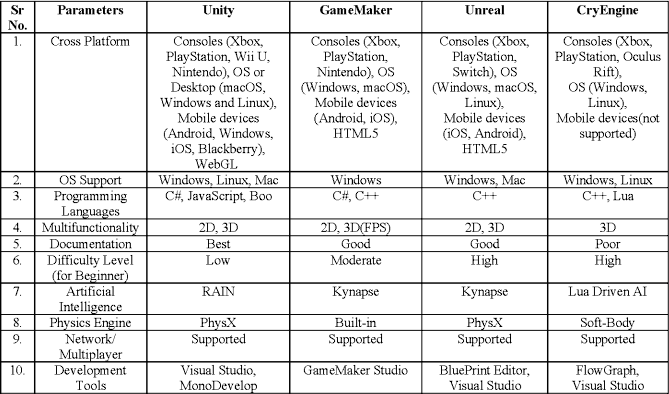
\includegraphics[width=0.9\textwidth]{images/GameEngineComparison.png}
    \caption{Game engine comparison, courtesy of \cite{9579618}}
    \label{image:gameEngineComparison}
\end{figure}
\pagebreak
\subsubsection{Graphics}
This is a big area of comparison between the two game engines, with Unreal engine being regarded very well in the industry for its very impressive graphics system due to its far more advanced rendering system compared to Unity that out of the box can produce much more impressive visual fidelity and finer looking results, however, this factor was not very important to me personally and as such, the increased graphical fidelity offered by the Unreal Engine was not a significant enough factor to affect my decision.
\subsubsection{Learning Value}
As the goal of the final year project is to further my own skills in software development according to my personal goals, one of the largest factors as regards choosing game engine was in fact the associated scripting language. I have a goal in the future to get a career in .net-based development and as such Unity's use of C\# was a major benefit for me in terms of learning the skills I desired to possess for my future career. And the fact that the C\# used in Unity isn't too dissimilar from standard C\# was a big bonus for me.
\section{Languages}
As mentioned earlier in the review language was a large factor in my choice for this project and the language that I intended to use was C\#. C\# is an object-oriented programming language developed by Microsoft which is used for developing desktop applications, games and web applications. It is frequently used to develop for Windows, iOS or Android. It is very heavily used in the software industry, according to a survey done by Stack Overflow in 2022, 29.7\% of developers claimed to use it \cite{stackOverflowSurvey2022}, meaning that it ranked as more popular than C and C++ in the same survey and less popular than Java.
\par
C\# is a strongly typed programming language, meaning that all variables must be declared with a specific type unless they are declared as either var or dynamic, variables specified as var will however still function as strongly typed and the type of variable is assigned at compilation based on how the variable is used. variables declared dynamic are instead resolved in run-time, however, I will not delve into these variables as I feel their use detracts from the advantage of a strongly typed language, that being that code is more readable and self-documenting, leaving less guesswork to the developer.
\par
As C\# is used with the .NET framework, it runs on the .NET Common Language Runtime which means that it avails of the CLR's built-in garbage collector. The presence of an in-built garbage collector ensures that I don't have to worry about the manual management of memory when writing code, it ensures that any unused objects will be cleared from memory avoiding memory leaks and improving the security of written code. The garbage collector works by checking if an object can be accessed through the application's code and if not, the memory used by the object is freed up, this behaviour can be modified using weak references, in that objects which can be accessed by code through a weak reference can still be collected using the garbage collector.
\subsubsection{Benefits of Object-Oriented Programming}
C\# is an object-oriented programming language, meaning that code is largely classed into classes and objects, this naturally complements game development very well as all the individual components making up a game can easily be thought of as objects, and the nature of object-oriented programming with each class containing its own associated data and methods makes it much easier to develop game components in a modular fashion and then integrate with each other.
\par
Additionally, aspects like encapsulation, meaning that the variables or properties that affect the internal state of an object can be isolated, meaning that we can ensure these instance variables that we wish to be private can only be accessed through the use of specific methods designed for classes. This makes the code more reliable and less bug-prone as it makes it easier to keep track of the different ways that objects can interact with one another.
\par
Other object-oriented principles such as polymorphism also make it easier to write more versatile code which can be modified in different ways depending on the particular goal, function overloading is the case that was most interesting to me, as with the purpose of the game being around evolution, there was the important aspect that the creatures in-game where e
\par
The object-oriented nature also made it easier to implement different performance-improving features that I figured would be necessary for the project, such as object pooling, which due to inheritance meant a generic object pool could be written to store any kind of game objects/
\section{Neural Networks}
In this chapter, I will be delving into Neural Networks which are an important aspect of my project. I will be writing a bit about them and several key aspects and justifying why in the end I chose to use a rather simple implementation of one.
\subsection{Introduction of Neural Networks}
Neural networks which at least in part were inspired by attempts at understanding the manner in which natural neurons operate and work in organic organisms. Neural networks are a broad class of machine-learning models which can be used to recognize patterns and create systems which can be trained to perform certain roles or tasks either using pre-obtained training data or through live feedback.
\par
Neural networks can be represented as directed graphs, and are most often composed of a variety of nodes or neurons which are linked together through connections which can have their own weights affecting the values of the outputs that they transmit.
The \ref{image:neuralNetworkStructure} provides a sample structure of a feed-forward neural network, meaning a network wherein there are no cycles formed by any looping connections between nodes. This sample structure is a neural network with an input layer, 2 hidden layers and an output layer.
\begin{figure}[ht!]
    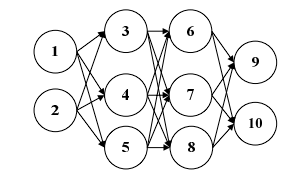
\includegraphics[width=0.9\textwidth]{images/NeuralNetworkStructure.png}
    \caption{Sample Structure of Feed-Forward Neural Network, courtesy of \cite{GURESEN2011426}}
    \label{image:neuralNetworkStructure}
\end{figure}
\par
I have included an image of a simple feed-forward neural network, as in the context of my project I intend only to include a small feed-forward neural network without even utilizing the advantages of more advanced training techniques like back-propagation as I feel that they don't fit in properly with the goals of my project.
\section{GitHub Copilot}
GitHub Copilot is an AI-powered coding assistant developed by a collaboration between GitHub and OpenAI. It is based on the Codex model developed by OpenAI \cite{OpenAICodex}, which itself was built upon the GPT-3 architecture. 
\subsection{Advantages of GitHub Copilot}
GitHub Copilot can offer developers intelligent suggestions as they type, anything from singles lines of code to entire blocks of code, which if using the Copilot extension in your IDE can simply be used with auto-complete, for example by using the tab key in Visual Studio.
\par
GitHub Copilot can also synthesize entire blocks of code or functions based on comments, taking the comments as suggestions and providing auto-complete suggestions that will meet the request.
\par
GitHub Copilot also displays an apparent ability to learn from context based on a user's project, with the suggestions becoming more accurate and appropriate to the work being done if the user engages with Copilot by accepting relevant suggestions and rejecting those that are inaccurate or irrelevant to the developer.
\par
An advantage of GitHub Copilot that was particularly relevant to me was that GitHub Copilot as of the time of writing this dissertation is available for free use by students, giving students an opportunity to get experience with GitHub Copilot for free so that we will likely grow accustomed to its use and continue to use in professional careers as software developers.
\section{Summary}
In Summary, I have decided that I will use Unity as my game engine for development, with C\# as the programming language of choice and that I will use a simple feed-forward neural network for controlling the creatures in my simulation.